%BEGIN_FOLD % Package includes
\documentclass[11pt,draftd]{article}
\usepackage{color}
\usepackage{hyperref}
\hypersetup{colorlinks, citecolor=green, filecolor=black, linkcolor=blue, urlcolor=blue }
\usepackage[a4paper, margin=1in]{geometry}
\usepackage{amsmath}
\usepackage{amssymb}
\usepackage{bm}
\usepackage{txfonts}
\usepackage{algorithm}
\usepackage{algorithmicx}
\usepackage{algpseudocode}
\usepackage{mathtools}
\usepackage{relsize}
\usepackage[titletoc,title]{appendix}
\usepackage[final]{pdfpages}
\usepackage{todonotes}
\usepackage{graphicx}
\graphicspath{ {images/} }
%END_FOLD
\setlength{\parindent}{0pt} % Remove indents

%BEGIN_FOLD % New definitions / commands

\makeatletter
\def\BState{\State\hskip-\ALG@thistlm}
\makeatother
\def\Real{I\!R}

\DeclarePairedDelimiter\abs{\lvert}{\rvert}
\DeclarePairedDelimiter\norm{\lVert}{\rVert}
% Swap the definition of \abs* and \norm*, so that \abs
% and \norm resizes the size of the brackets, and the 
% starred version does not.
\makeatletter
\let\oldabs\abs
\def\abs{\@ifstar{\oldabs}{\oldabs*}}
\let\oldnorm\norm
\def\norm{\@ifstar{\oldnorm}{\oldnorm*}}
\makeatother

% New definition for Lagrange symbol
\newcommand{\Lagr}{\mathcal{L}}

% New definitions for bold texts
\newcommand{\bfB}{\mathbf{B}}
\newcommand{\bfA}{\mathbf{A}}
\newcommand{\bfPsi}{\mathbf{\Psi}}
\newcommand{\bfPhi}{\mathbf{\Phi}}
\newcommand{\bfK}{\mathbf{K}}
\newcommand{\bfP}{\mathbf{P}}
%END_FOLD

\begin{document}
% TITLE PAGE -----------------------------------------------------------%
%BEGIN_FOLD
\title{High-performance UAV motion planning and control for passage through tight gaps}
\author{David Dos Santos}
\date{BEB801 - Project 1}
\maketitle
%END_FOLD

% EXEC SUMMARY ---------------------------------------------------------%
%BEGIN_FOLD
\[\]
\[\]
\[\]
\renewcommand{\abstractname}{Executive Summary}
\begin{abstract}
	\[\]
	This project aims to contribute to the knowledge of optimal control, especially in the field of high performing computational algorithms for solving optimal control. The problems being considered and tested are stochastic and non-linear. A key area within this field is dynamic programming which suffers from the curse of dimensionality. This project seeks to utilise new approaches to overcome the barrier of the curse of dimensionality and improve the performance of numerical methods on complex problems. \\
	
	\noindent A novel approach has been presented which utilises a continuous linear algebra technique, known as the tensor decomposition. It claims to improve the compression of the control optimal solution as well as to reduce the computational complexity. A comparison study will be conducted with this new approach against a well-known and highly accurate method: the Markov Chain Approximation. To approach the comparison study, a library for utilising the Markov Chain Approximation will be developed. A library for using the tensor decomposition method has already been developed for Unix based systems. Using a known problem and a UAV simulation test bed, the two methods will have their computational speed and storage efficiency compared. \\
	
	\noindent A schedule has been proposed to break this project down into manageable tasks. This report shows the current progress in this schedule and any adjustments needed to be made. If significant progress is made in the schedule, then deployment into a real/physical environment will be sought after. \\
	
	\noindent Previous to this report, a project proposal and a literature assortment were conducted. The literature assortment was paramount to the development of this research topic and project scope. It also helped to find the tensor decomposition method and library which meant that time on the schedule did not need to be allocated towards writing another library, but instead, only on learning how to use it. The project proposal helped to define the scope of this research project, and part of that proposal's work has been reflected in this report. \\
	
	\noindent This report in its current state reflects the progress that has been achieved thus far. It also analyses the alignment of the previously proposed schedule to the actual task accomplishment. Adjustments are considered and proposed as appropriate.
	\todo{Fix exec summary}
\end{abstract}
\pagenumbering{gobble}
%END_FOLD

% TABLE OF CONTENTS ----------------------------------------------------%
%BEGIN_FOLD
\clearpage
\pagenumbering{roman}
\setcounter{page}{1}
\renewcommand{\contentsname}{Table of Contents}
\tableofcontents
\newpage
%END_FOLD

% ASSIGNMENT -----------------------------------------------------------%
\clearpage
\pagenumbering{arabic}
\setcounter{page}{1}

\section{Introduction}
There have been significant advancements in the combined fields of mathematics and control systems engineering over the last century. Advanced control systems are fundamental to emerging technologies for many engineering fields, such as aeronautics and automation. Thus, this research project began with looking into the challenges of solving optimal control problems, and works towards improving the techniques often used to solve them. \\

The optimal control problems being considered in this project, are in nature, difficult to solve with mathematical analysis. For example, the manoeuvring of a UAV flying through a tight gap is best accomplished by calculating and storing an optimised motion plan and control scheme of the UAV's systems. Such a problem is non-linear and has stochastic processes involved (e.g. turbulent wind), and is part of the motivation for this project. Therefore, we seek rather to solve these complex problems using computational mathematics. \\

Such numerical techniques can take advantage of the ever-growing processing power and speed of modern computers. Yet, for a lot of these problems the underlying algorithms turn out to be computationally challenging with an increase in dimensional state-spaces: known as the \textit{curse of dimensionality} \cite{dynamicprogramming}. Meaning, its computational expense grows exponentially with the number of degrees of freedom used in the problem.\\

Simply designing and building faster, and more powerful computers will not be sufficient to solve this computational concern \cite{powersystem}. New computational methods must be developed based on superior control architectures and new algorithms. Having a deeper understanding of emerging relevant research in this field can help us to see this. If we can overcome the barrier of the \textit{curse of dimensionality}, then we will have greatly benefited the fields of not only computational mathematics, but also the areas of aerospace automation, architecture, electrical smart grids, data management, modelling, and security.\\

\subsection{Research Aims and Objectives}
A novel approach in continuous computational linear algebra has been developed by Alex Gorodetsky \cite{alex-c3}, known as the tensor decomposition method. It claims to improve upon the performance of solving non linear stochastic control problems and suggests that it can even mitigate the curse of dimensionality. Thus, this project aims to prove this hypothesis through a comparison study. The comparison will involve testing the accuracy and efficiency of this novel approach against another well-known method: the Markov Chain Approximation (MCA) \cite{kushner}. \\

Specific examples will be investigated: a one-dimensional optimal control problem to begin (see Section \ref{1dproblemdefinition}), and then an extension to a higher dimension stochastic optimal control problem. \\

Some key questions that is sought to be answered from this research are:
\begin{enumerate}
	\item Is the novel tensor decomposition method more computationally efficient?
	\item How much accuracy is lost from using this method? Is it a feasible approach?
	\item What are the requirements, or specific scenarios, that this tensor decomposition works for?
	\item When is it more appropriate to use the tensor decomposition method over other well-known approaches? And when is it not best to use it?
\end{enumerate}
\newpage

\section{Project Description}
\subsection{Project Deliverables and Outcomes}
This research project contributes to the knowledge of optimal control, especially in the field of optimal control solutions for stochastic non-linear problems. Through this study, a greater understanding into numerical methods for these high-dimension state spaces will also be achieved. 
The deliverables at the end of this research project will be:
\begin{itemize}
	\item A fully documented MCA software library
	\item A MCA script which uses the above library to solve stochastic non-linear control problems (given as an example to show how to use the library, and to help with comparison studies)
	\item A Tensor Decomposition script which uses the “C3” open-source library \cite{c3c} (given as an example to show how it can be used to solve our stochastic optimal control problems, and to help with the comparison studies)
	\item A report showing a verification and comparison study between the two approaches
\end{itemize} 

Outcomes expected to be achieved in this project are:
\begin{itemize}
	\item Increased understanding of dynamic programming methods
	\item High performance ability to solve a UAV motion plan and control system for passage through tight gaps
\end{itemize}

\subsection{Requirements / Specifications}
In order to clarify the scope of the project objective and deliverables, requirements and specifications have been set:

Hence, the delivered libraries must be intuitive and documented appropriately, allowing future work to easily carry on. For the software package to be viable, it needs to meet the following specifications:
\begin{itemize}
	\item The delivered software must be able to solve a variety of control problems. For this reason, it was considered best to produce software libraries which can be adapted for many different scenarios and problems (relating to stochastic nonlinear control).
	\begin{itemize}
		\item The library must be intuitive and fully documented - allowing future work to easily carry on
		\item The proposed language to use for the library is C++.  The proposed language to use for the MCA software is C++. This language was designed with a bias toward embedded, resource-constrained systems (like micro controllers), with performance, efficiency and flexibility of use as its design highlights \cite{c++film}. Because the C3 library is written in the language of C, using the language of C++ will also allow for simple cross-code portability as necessary.
	\end{itemize}
	\item Completed software scripts should be capable of running and producing a solution on a standard Unix based system. The standard computer is considered to have the following minimum specifications:
	\begin{itemize}
		\item Ubuntu 16.04 operating system (64 bit)
		\item 8GB of Ram
		\item Intel i5 Processor (quad-core), (Haswell code-name)
	\end{itemize}
	\item The software should require no more than the allotted 8gb of RAM and execute completely in under 60 minutes
	\item The resulting solution to this script should also exist in a file which is no larger than 8GB (allowing it to fit into a USB and be transported easily)
\end{itemize}

\noindent

\subsection{Approach / Methodology}
To approach the comparison study, there needed to be a library for accessing and testing both methods. Fortunately, a library for using the Tensor Decomposition method has already been completed and openly shared \cite{c3c} \cite{c3cs}. Thus, first an MCA software library was to be written for a one dimensional case. From this, the two methods would be tested and confirmed to be accurate using a problem with a known solution. Testing of computational efficiency is not as applicable at this stage but would be conducted nonetheless.\\

Following this, the MCA library would be further developed to account for problems of a higher dimension. Then the two methods will be compared on a complex problem using a provided UAV simulation test bed. This test would compare computational storage needed, time taken to compute, and accuracy of the results. See the following figure for a visual depiction of the overall tasks.

\begin{figure}[h]
	\centering
	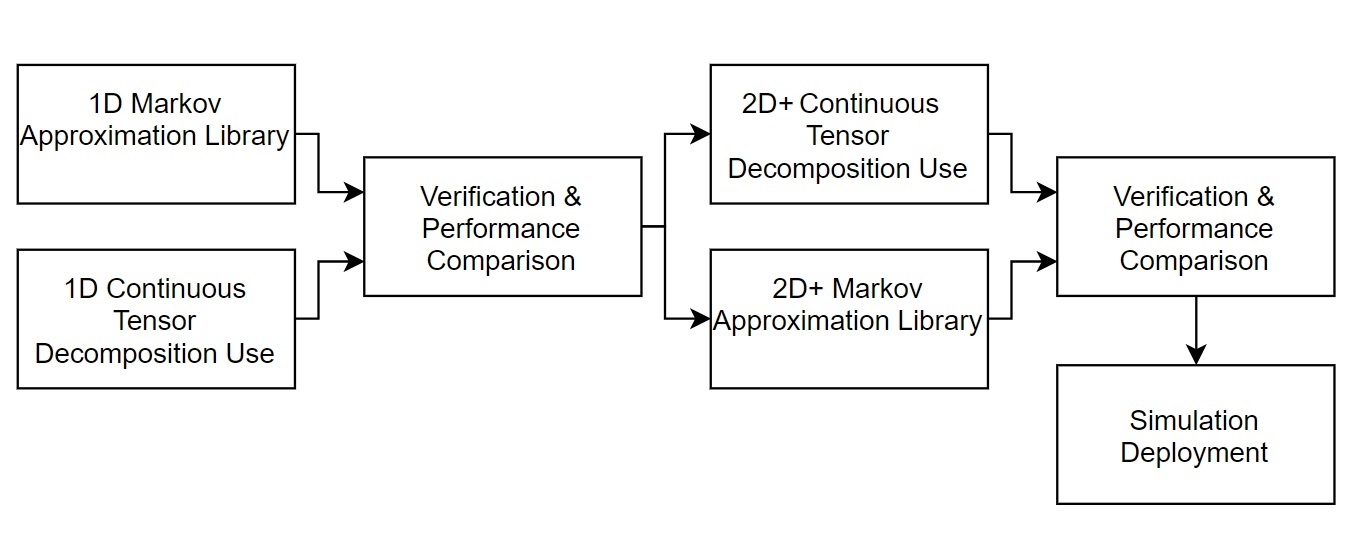
\includegraphics[scale=0.4]{WorkBreakdownMethodologyFigure}
	\label{WorkBreakdownMethodologyFigure}
	\caption{Section Breakdown of Methodology}
\end{figure}

The aforementioned steps were broken down into manageable tasks, and can be seen in the Appendix under Item \ref{app_itemB} - Work Breakdown structure. Current progress along this timeline is given in Section \ref{ProjectProgress} Project Progress (see page \pageref{ProjectProgress}). If significant progress is made in the schedule, then deployment into a real/physical environment will be sought after.
\newpage
\section{Literature Review} 
\subsection{Background to Optimal Control}
\todo{Weak description of dynamic programming}
A control system consists of subsystems and processes assembled for the purpose of obtaining a desired output with desired performance, given a specified input \cite{nise}. Our interest lies in the topic of optimisation, known as the field of optimal control: to find the mathematical optimisation for control problems \cite{ieeeControl}. An optimal control is usually represented in a set of differential equations describing the paths of the control variables that minimise the cost function -- a mathematical formula used to graph the cost of an application or process given certain inputs \cite{costfunction}. \\

The optimization of control problems arises in many settings, ranging from efficiently managing heating systems to improving entire economies \cite{powell}. Other examples include: effective aircraft landing, managing large stock of blood inventories, scheduling numerous fleets of vehicles, selling assets, planning and integrating large electrical grids, and even playing a game of tic-tac-toe or backgammon. Each of these problems involve making decisions, then observing results, followed by more decision making and so on. Although such problems can sometimes be straightforward to formulate, they are not always as simple to solve. \\

Dynamic programming is a method for solving complex optimisation problems: by breaking it down into a collection of simpler sub problems - solving each of those sub problems just once, and storing their solutions \cite{wikiDyn}. Ideally, this method is best built using a memory-based data structure - then on the next occurrence of the same sub problem, the computed solution already exists and is not required to be recalculated. This tactic can save computation time at the expense of storage space. In the dynamic programming approach, we seek an optimal value function that is equal to the optimal cost function. In continuous-time and space, the optimal value function is the solution to the Bellman equation. \todo{reference}\\

\subsection{Contribution to Modern Control Systems}
Dynamic programming is the approach we have decided to use in solving complex problems. Unfortunately, it comes with something called the curse of dimensionality, and if we can improve upon this barrier then the future of engineering within optimal control can be greatly benefited. \\

This curse of dimensionality basically means that the computational complexity (and hence, the run-time) for solving dynamic programming problems grows exponentially with the number of dimensions considered in the state space. So, for complex problems such as motion planning for a UAV through a tight gap, the time taken to numerically solve it is far too long and the memory storage needed to store the solution is far too high. Rather than attempting to overload our available computational power, we are to look at evolving the current methods being utilised. \\

A well-known numerical method for solving optimal control problems is the Markov Chain Approximation (MCA) \cite{kushner}. The basic formula of the MCA is to approximate the original controlled process by a chosen controlled Markov process within a finite state-space (effectively it is a “discretisation” of the original state space of the problem). \\

\subsection{Novel Tensor Decomposition Approach}
A novel approach has been presented which utilises a tensor decomposition technique to improve the compression of the optimal solution as well as to reduce the computational complexity. This approach is termed as \textit{compressed continuous computations} (C3) and extends from the \textit{continuous computation} framework, which roughly refers to computations with functions instead of discrete arrays, and was employed in the popular Matlab software package Chebfun. In the Chebfun software package, the user performs computations using uni-, bi-, or tri-variate functions which are represented in Chebyshev polynomial bases \cite{chebfun}. The tensor decomposition carries on from the research conducted of the ‘Function-Train’ \cite{ft-alex}.

Some of the advantages to this approach are:
\begin{itemize}
	\item Continuous input space of a high-dimensional function, rather than a discretised set of inputs (far less storage space required)
	\item Fast adaption to local features of a function, rather than iterative grid refinement methods
	\item Continuous multi linear algebra techniques which enable fast addition, multiplication, contraction, integration, differentiation and other useful operations
\end{itemize}
By utilising this new approach, the time taken, and storage needed, to numerically solve a non-linear stochastic control problem (such as that of the UAV manoeuvring through tight gaps) can hopefully be reduced significantly. This is also hoped to be accomplished without losing needed accuracy.\\

\subsubsection{Continuous Linear Algebra}
As noted, the fundamental backbone of the tensor decomposition algorithm lies in interpreting continuous objects on a computer not as being discretised but rather parametrised. Usually discretisation implies that the computer can only “see” a function on a computer through its evaluation at a set of points. Parametrisation implies that the computer can “see” a function on a computer through a finite set of parameters and a set of routines that map those parameters to outputs of interest \cite{thesis}. In discrete linear algebra, the primary elements of dynamic programming equations are vectors and matrices. But in this continuous linear approach the primary elements are scalar-, vector-, and matrix-valued functions. The following figure shows how this difference was applied in the C-programming language.

\begin{figure}[h!]
	\centering
	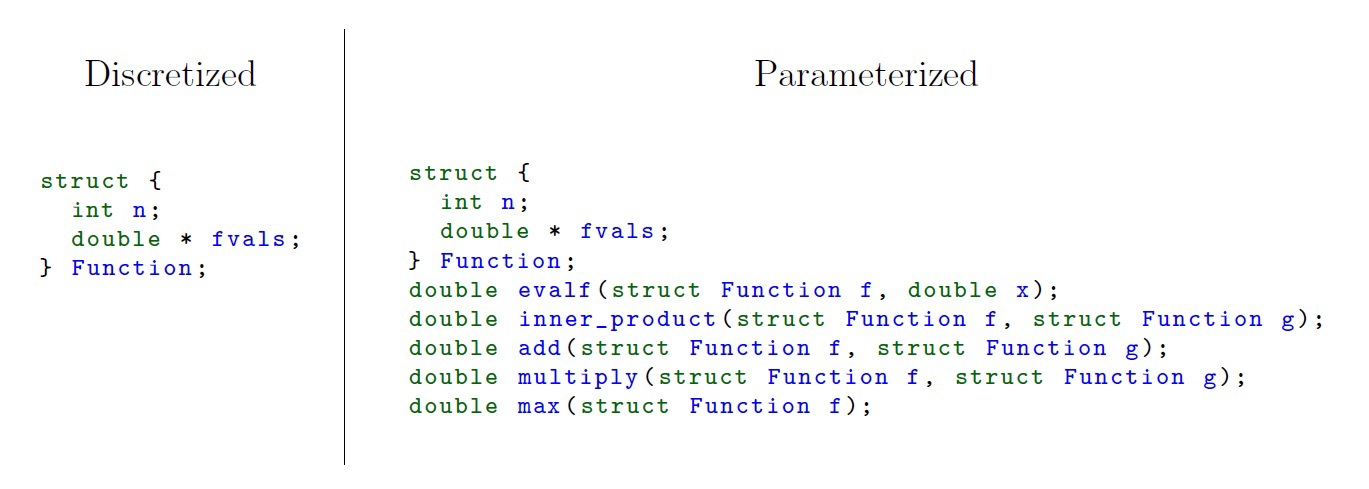
\includegraphics[scale = 0.4]{ContinuousLinearAlgebraDifference1}
	\caption{Parameterisation affect and application in C-programming language}
\end{figure}

\subsubsection{Function Train Construction}
To extend the Chebfun functionality in computing multivariate functions, it was important to represent them en a scalable manner that tackles the curse of dimensionality. Specifically, the C3 framework seeks to represent multivariate functions in a format where the cost of storage grows polynomially, instead of exponentially, with dimension. Furthermore, representations and associated algorithms were designed to scale with a functions "rank" rather than the number of inputs. Thus algorithms were developed for converting to, and computing functions in a low-rank format called the \textit{function-train} decomposition.

An function-train (FT) is defined by a set of $ d $ matrix-valued functions $ \{\, \mathcal{F}_{1}(x_{1}),\cdots,\mathcal{F}_{d}(x_{d}) \,\} $, and a set of FT-ranks $ \bm{r} = [r_{0},\cdots,r_{d}] $ where $ r_{0} = r_{d} = 1 $ and $ \mathcal{F}_{i} : [a_{i}, b_{i}] \rightarrow \mathbb{R}^{r_{i-1}\times r_{i}} $ for $ i = 1, \cdots, d $. Furthermore, an evaluation of a function $ f (x) $ in FT format is obtained through a sequence of vector-matrix products:
\begin{align*}
	f(x) = \mathcal{F}_{1}(x_{1})\mathcal{F}_{2}(x_{2}) \cdots \mathcal{F}_{d}(x_{d}) 
\end{align*}
It is also helpful to think of these as matrices of univariate functions, like so:
\begin{align}
	f(x) = \begin{bmatrix}
	f_{1,1}^{(1)} & \cdots & f_{1,r_{1}}^{(1)}
	\end{bmatrix}
	\begin{bmatrix}
	f_{1,1}^{(2)} & \cdots & f_{1,r_{2}}^{(2)} \\
	\vdots & & \vdots \\
	f_{r_{1},1}^{(2)} & \cdots & f_{r_{1},r_{2}}^{(2)}
	\end{bmatrix} 
	\cdots
	\begin{bmatrix}
	f_{1,1}^{(d)} \\
	\vdots \\
	f_{r_{d-1},1}^{(d)}
	\end{bmatrix}
\end{align}

The operations of addition, multiplication, differentiation, integration, and inner products are easily performed for functions in FT format \cite{thesis}. 
\newpage

\section{Project Development} \label{ProjectProgress}
\subsection{Work Breakdown Overview}
This research project followed a project plan which been given previously in the work breakdown structure. The full detail of this can be found in the Appendix under Item \ref{app_itemB} - Work Breakdown structure. \\

In order to establish the validity of the novel tensor decomposition approach, this new method must be tested against a known method (the MCA method) and compared using a sufficiently difficult problem. To begin, a simple problem with a known solution will be used to ensure that both libraries give the same results (deducing their validity). Because the C3 framework library was already constructed, a significant portion of time in this research project was allocated to developing an MCA library. \\

Fortunately, the library for using tensor decomposition techniques has already been developed and freely given as open source (see \cite{c3c} and \cite{c3cs}). The main library's abbreviated name is C3, and the extension library’s abbreviated name is C3SC (the 'SC' referring to stochastic control). Together they allow for fast computations of stochastic optimal control problems using a continuous tensor decomposition method. \\

Difficulties prevented the full realisation of this plan and hence it was clearly important to help alleviate these problems from future work, and thus a Git repository has been created which has the MCA library (with examples), and automated download scripts for the C3 library. This Git repository can be found at \url{https://github.com/revolutionized/High-Performance-Control/}. \\

To avoid the installation problems in the future, a user manual was also generated which covers a step-by-step installation of all necessary components for the MCA and C3 libraries to work (on any of the three major operating systems: Windows, MacOS, and Ubuntu). The user manual is included in the Git repository. A documentation of the MCA C++ classes has also been auto-generated using \href{https://www.stack.nl/~dimitri/doxygen/}{Doxygen}, explaining the layout and usage of the code. An example of this documentation can be seen in the following figure. \\
\todo{update doxygen figure}
\begin{figure}[h!]
	\centering
	\label{doxygen-documentation}
	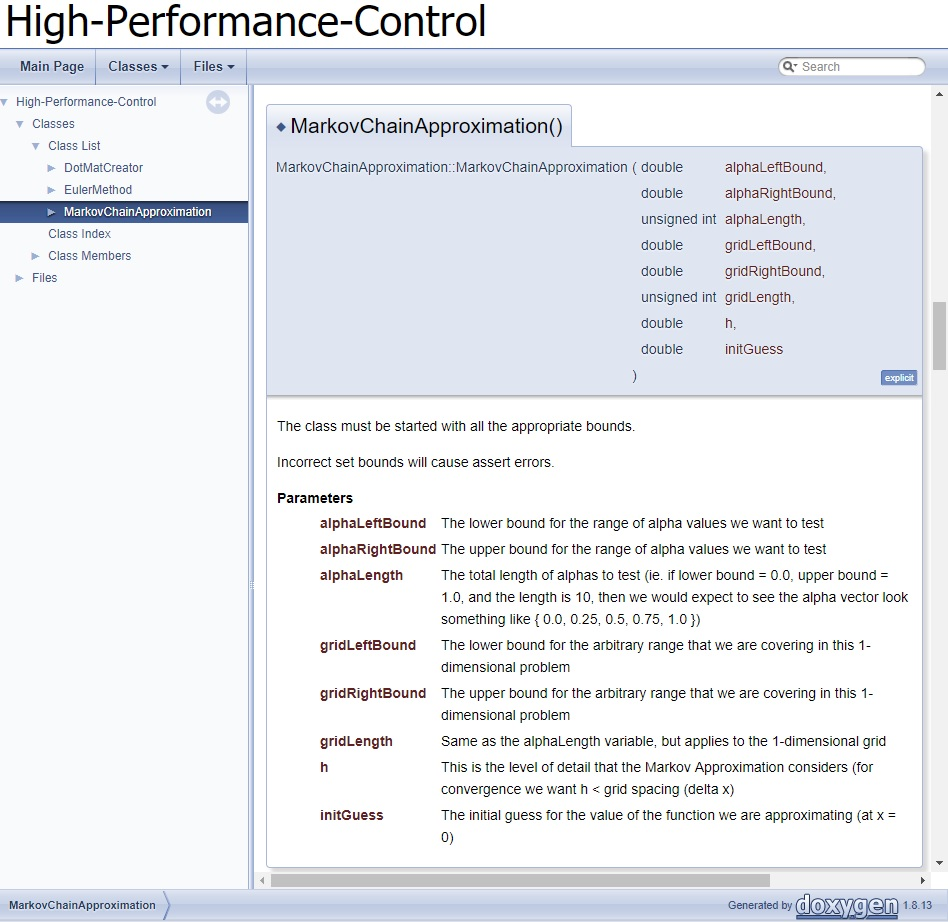
\includegraphics[scale = 0.63]{doxygen-example}
	\caption{Autogenerated documentation of code}
\end{figure}
\[\]

\subsection{Literature Assortment}
The first step of this research project was a topic investigation. For that, the following steps were taken:
\begin{enumerate}
	\item A concept map was drawn which defines the topic
	\item A search statement was developed and used to find the most relevant literature
	\item Engineering databases were researched and the most relevant databases were selected
	\item Information sources (such as conference publications, international journals, engineering texts and standards) were identified
	\item 3 key literatures were reviewed which matched that of the topic investigation - and from this the project proposal scope was formed
	\item Published authorities in the chosen field of dynamical stochastic control were also cited	
\end{enumerate}
This literature assortment was paramount to the development of this research topic and project scope. It also helped to find the Tensor Decomposition library which means that time on the schedule did not need to be allocated towards writing another library but only on learning the library (which in comparison would be far less). \\

\section{Developing the Markov Chain Approximation}
As noted in the Work Breakdown Structure, it is noted that the initial phase of this project gave time for learning and developing a library for the MCA method. In \cite{kushner}, we learn the mathematical construction required for the MCA.  \\

The basic process to constructing the MCA is as follows
\begin{enumerate}
	\item Approximate the original problem with a simpler stochastic process model and its associated cost function
	\item This stochastic process is a Markov chain on a finite state space (which is a discretisation of the original state space)
	\item A cost function for the Markov chain model is found
	\item MCA is parametrized by a parameter, $ h $, (the finite element size), such that, as the parameter goes to zero, the chain resembles more and more closely the original problem
	\item Then numerical techniques can be utilised to solve the stochastic process (which resolves to the original problem as the parameter, $ h $, goes to zero)
\end{enumerate}
\[\]
\subsection{Mathematical Construction of Markov Chain Approximation}
The method used and discussed here is the "finite difference" method. I begin with a one dimensional example with control, and later considered a general $ n $-dimensional case with one control parameter.

\subsubsection{One Dimension with Control}
The following is the mathematical derivation / construction of the Markov Chain Approximation algorithms. \\

We begin by letting the control $ u $ be of the feedback type, and let $ x $ be defined by:
\begin{equation}\label{Eq_PduDefinition1D}
	dx(t) = b(x(t),u(t)) dt + \sigma(x(t))d\omega
\end{equation}
Where $ b(x,u) $ is the drift term of the system, $ \sigma(x) $ is the diffusion term of the system, and $ d\omega $ is a Weiner stochastic process. This code derivation was first realised in \cite{kushner}, and is the backbone to the code construction. \\

Now, let the first escape time of the sequence be defined as $\tau = \min\left(t : x(t)  \notin \left(0, B\right)  \right) $. Hence, define the cost function as:
\begin{align}\label{W_x_u}
	W(x,u) &= E_{x}^{u}\left[\int_{0}^{\tau}k(x(s),u(x(s)))ds + g(x(\tau))\right] \\
	W(x,u) &= g(x),\; \text{for } x=0,B
\end{align}
By applying It$\hat{\text{o}}$'s formula to the function \eqref{W_x_u}, it yields the equation:
\begin{align}\label{Eq_Lagrange1D}
	\Lagr^{u(x)}W(x,u) + k(x,u) = 0, \quad x\in(0,B)
\end{align}
with boundary conditions $ W(0,u) = g(0) $, $ W(B,u) = g(B) $. And where $ \Lagr^{\alpha} $ is the differential operator of $ x $ when the control is fixed at some value, $ \alpha $. \\

To get a consistent Markov chain and interpolation interval, we simply use the finite difference approximations as follows
\begin{align}
	f_{xx}(x)\;\;&=\;\;\frac{f(x+h) + f(x-h) - 2f(x)}{h^{2}} \\
	f_{x}(x) \;\;&=\;\;\frac{f(x+h) - f(x)}{h} \qquad \text{if $ b(x) \ge 0 $} \\
	f_{x}(x) \;\;&=\;\;\frac{f(x) - f(x - h)}{h} \qquad \text{if $ b(x) < 0 $}
\end{align}

for the $ W_{xx} (x,\alpha)$ and $ W_{x} (x,\alpha)$ in \eqref{Eq_Lagrange1D}. \\

Now define the transition probabilities, $ p^{h} $, for a controlled Markov chain. Also define the interpolation interval, $ \Delta t^{h} $, where $ \Delta t^{h} > 0$. We can formulate the following:
\begin{align}
	p^{h}(x,x\pm h|\alpha) &= \frac{\sigma^{2}(x)/2 + hb^{\pm}(x,\alpha)}{\sigma^{2}(x)+h\abs{b(x,\alpha)}} \label{Eq_ph} \\
	\Delta t^{h}(x,\alpha) &= \frac{h^{2}}{\sigma^{2}(x) + h\abs{b(x,\alpha)}} \label{Eq_Deltat}
\end{align}
We must also set $ p^{h}(x,y|\alpha)=0 $ for $ y\ne x\pm h $. We can also follow a procedure to show that:
\begin{equation}\label{Eq_Wsum}
	W^{h}(x,u) = \sum_{y}p^{h}(x,y|u)W^{h}(y,u) + k(x,u)\Delta t(x,u)
\end{equation}
And hence, if \eqref{Eq_Wsum} has a unique solution then it is the cost associated with the controlled chain. \\
Now we arrive at the dynamic programming equation for the optimal value function:
\begin{equation}\label{Eq_dynamicV}
	V^{h}(x) = \min\left[\sum_{y}p^{h}(x,y|\alpha)V^{h}(y) + k(x,\alpha)\Delta t^{h}(x,\alpha)\right]
\end{equation}
Which has the same boundary conditions as for \eqref{W_x_u}. \\

Authors of \cite{kushner} emphasises that no claim is made that the convergence of the finite difference approximations can be proved via the classical methods of numerical analysis. Rather, they suggest that the finite difference approximation is used primarily to get the transition probabilities of a Markov chain which is consistent with \eqref{Eq_PduDefinition1D}. \\

To further improve performance of this approximation method, we notice that the presence of the control parameter $ \alpha $ in the denominators of the expressions for the transition probabilities and interpolation interval in \eqref{Eq_ph} and \eqref{Eq_Deltat} can complicate getting the solution of \eqref{Eq_dynamicV}. And thus, one simple way of eliminating the dependence of the denominators is to define $ B(x) = \max\abs{b(x,\alpha)} $. Which yields:
\begin{align}
	\bar{p}^{h}(x,x\pm h|\alpha) &= \frac{\sigma^{2}(x)/2 + hb^{\pm}(x,\alpha)}{\sigma^{2}(x)+hB(x)} \label{Eq_phat} \\
	\Delta \bar{t}^{h}(x,\alpha) &= \frac{h^{2}}{\sigma^{2}(x) + hB(x)} \label{Eq_Deltathat}
\end{align}
The difference between the barred and unbarred values is of order $ O(h) $. \\

To calculate the control at each iteration, we get an approximate value for $ W(\cdot,u_n) $ and then solve the following
\begin{equation}
u_{n+1}(x) = \arg\min_{\alpha}\left[\sum_{y}\bar{p}^{h}(x,y|\alpha)W^{h}(y,u_{n}) + k(x,\alpha) \Delta\bar{t}^{h}(x,\alpha)\right]
\end{equation}
Where our cost function is:
\begin{equation}
W^{h}(x, u_{n}) = \sum_{y}\bar{p}^{h}(x,y|u_{n}(x))W^{h}(y,u_{n}) + k(x,u_{n}(x)) \Delta\bar{t}^{h}(x,u_{n}(x))
\end{equation}

\[\]
\subsubsection{Pseudo-Code For one Dimension}
The following Pseudo-Code was developed in according with task 1.1 of the Work Breakdown Structure. They show the computational algorithm needed to construct an MCA, and solve an optimal control problem. Currently the Pseudo-code is set up to work for a one dimensional stochastic model with control (see Equation \eqref{Eq_PduDefinition1D}). \\

The Initial Setup algorithm sets out all necessary parameters needed for the MCA.

\begin{algorithm}[H]
	\label{alg-setup}
	\caption{Initial setup}
	\begin{algorithmic}[1]
		\Procedure{InitScenario}{}
		\State $\varepsilon \gets \text{set to a very small small value}$
		\State $\alpha \gets \text{guess range of control paramter} $
		\State $h \gets \text{set to a small positive value} $
		\State $ x \gets \text{discretise to segments of width } h$
		\State $ V_0 \gets \text{set initial guess} $
		\State Run \textbf{Algorithm 2}
		\EndProcedure{}
	\end{algorithmic}
\end{algorithm}

% Pseudo code - main loop
\begin{algorithm}[H]
	\label{alg-mainloop}
	\caption{Approximating Markov Chain}
	\begin{algorithmic}[1]
		\Repeat
			\ForAll{values of $ x $}
				\If{$ x $ is on boundary}
					\State Apply BC's and continue to next iteration of $ x $
				\EndIf
				\State $ y $ \Comment{determine the state $x$ can move to: $\pm h$}
				\For{each $ \alpha $}
					\State $ \Delta\bar{t}(x,\alpha)$ \Comment{solve normalised interpolated time} 
					\State $ k(x,\alpha)$ \Comment{compute cost using specified control} 
					\For{each $ y $}
						\State $ \bar{p}(x,y \vert \alpha) $ \Comment{solve normalised transition probability Markov chain}
						\State   \Comment{create array of probability transitions and}
						\State $ V_{n+1}^{h}(x,y,\alpha) = \bar{p}^{h}(x,y \vert \alpha) \times V_{n}^{h}(x,y,\alpha) \text{\hspace{2.1em}previous dynamic equation values}$
					\EndFor
				\EndFor
				\State \Comment{sum array, add instantaneous cost}
				\State \hspace{23em} and find the $\alpha$ which minimises
				\State $ V_{n+1}^{h} (x) = \min\limits_{\alpha}\left[ \mathlarger{\sum\limits_{y}} {V_{n+1}^{h}(x,y,\alpha)} + k(x,\alpha)\Delta\bar{t}^{h}(x,\alpha) \right] \text{\hspace{2.7em} the dynamic equation}$
				\State Store minimising $ \alpha $
			\EndFor
		\Until{$ \norm{V^{h}_{n+1} - V^{h}_{n}}_{\infty} \le \varepsilon \gets \text{check for dynamic equation convergence}$}
	\end{algorithmic}
\end{algorithm}
The above algorithm is for the solving of the dynamical programming equation $ V(x) $. From here, Euler's method is employed to solve the differential system, while using the control value that minimised the dynamic equation of the MCA. \\

\subsubsection{One-Dimension Problem Definition} \label{1dproblemdefinition}
The 1-D problem I decided to test against was a simple cart brake control problem which is defined below. \\

We consider a cart of mass $ m $ and linear viscous coefficient $ d $, which is acted by a control force $ F $. We will focus on the dynamics for the velocity $ v $. From Newton's 2nd law, it follows that
\begin{equation*}
	m\dot{v}=F-dv
\end{equation*}
If we define $ x = v $ and $ u = F $, then the above model can be represented as
$ \dot{x} = Ax + Bu$
Where $ A = -b/m $ and $ B = 1/m $. To begin, we choose the parameter values of $ m = 1\,kg$ and $ b = 2 $ Ns/m. We seek the optimal control law that minimises the following cost
\begin{equation*}
	J(x_0, u) = \int_{0}^{\infty}(5x^{2} + u^{2}) dt
\end{equation*}

This particular example has been chosen because it has a known solution that we can test and confirm our results against. The solution can be solved by using a Linear Quadratic Regulator (LQR). A brief has been given on the construction of the LQR formulation and use in Appendix Item \ref{app_itemC} - Brief on Linear Quadratic Regulator). \\

Using the LQR approach, we have $ A = -2,\, B = 1,\, Q = 5,\, R = 1 $. Then we use these values in the Riccati equation to get
\begin{align*}
	-S^{2}-4S + 5 &= 0 \\
	\therefore S &= 1
\end{align*}
The controller is 
\begin{equation*}
	u = -Kx
\end{equation*}
where $ K = R^{-1}(B^{T}S) = 1 $, thus the resulting closed-loop system is
\begin{equation*}
	\dot{x}^{\star} = (A - BK) x^{\star}  \qquad \therefore \dot{x}^{\star} = -3x^{\star}
\end{equation*}
Given an initial condition, $ x_0 $, our solution to this ODE is
\begin{equation*}\label{key}
	\dot{x}^{\star}(t) = x_{0}e^{-t/3};
\end{equation*}
And the optimal cost is 
\begin{equation*}
	J^{\star}(x_0) = x_{0}^{T}Sx_{0}=x_{0}^{2}
\end{equation*}
\[\]

\subsubsection{Initial Script in MATLAB}
During the course of the first semester, time had been put aside to learn the basics of the MCA method. The ultimate goal was to implement the method in the programming language of C++, as the currently existing library of C3 was written in C. But to begin, a test algorithm of the MCA method was written in MATLAB to ensure the MCA algorithm previously discussed was correct. MATLAB also was chosen because of its easiness in creating code and testing results. \\

The first step taken was to recreate an approximation to the solution using Euler's method. The results can be seen in the next two figures. Upon successfully completing this, the next task was to approximate the optimal control using the MCA method. Figure \ref{eulersmethod2} shows what value to set the control value to in order to minimise the cost function. The $ y $ axis is the level of the control variable, and the $ x $ axis is time in seconds. Where as figure \ref{eulersmethod1} shows the state of the carts velocity over time. Again, the $ x $ axis is time in seconds and this time the $ y $ axis is the one-dimensional velocity. Obviously when the brakes are applied with an exponential decay, we would expect the carts rate of slowing down to be an exponential decay. 

\todo{change figure so it doesn't have euler's in it}
\begin{figure}[h!]
	\centering
	\label{eulersmethod1}
	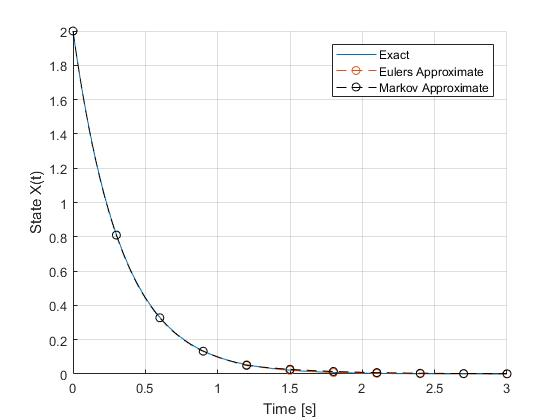
\includegraphics[scale = 0.6]{EulersApproximateState}
	\caption{Euler's approximation method results}
\end{figure}
\begin{figure}[h!]
	\centering
	\label{eulersmethod2}
	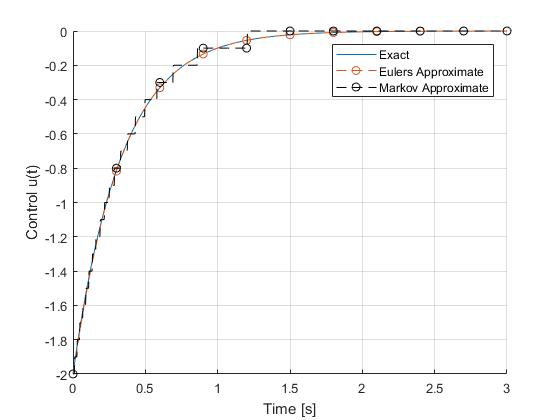
\includegraphics[scale = 0.6]{EulersApproximateControl}
	\caption{Euler's approximation method results}
\end{figure}

In the above figures, the 'Exact' plots refer to the MATLAB computed result of the solution to the given ODE. The 'Markov Approximate' plot is obviously the results generated from using the MCA method to find the minimum control, followed by the Euler's method to solve the differential system.

The MCA method initially ran into some code bugs which delayed the proposed finishing time of this task. But early this semester the bug was eradicated. It should also be noted that the Markov Approximation method obviously had a discretised solution (as can be seen from it's stepwise change) for the optimal control, but when looking at the state graph it obviously had little impact on the solution to the ODE. \\

\subsubsection{Script in C++}
Early this semester I began porting the MATLAB script and MCA method over to the C++ language. This was done so that easy integration could be made with the C3 library. Several C++ classes were made to separate the code into more manageable segments: \\
\begin{itemize}
	\item The EulersMethod class was created to perform Euler's method on a generic first order ODE. The user simply has to pass it the derivative of the ODE as a function and it will calculate everything needed for a 2-d plot.
	\item The DotMatCreator class was created to convert the Euler approximation result (or any 2-d array) into a format that MATLAB can use. However, the current script utilises Gnuplot instead - an open source graphing tool.
	\item The MarkovChainApproximation class was obviously created to implement the MCA method. The algorithms are hidden in the class so that all the user needs to do is give the range of parameters to use (as per Algorithm 1 from Section \ref{alg-setup}), and then call the ComputeMarkovApproximation method, giving it a cost function and a stochastic function. The MCA method here is based off the 1D problem definition given before. \\
\end{itemize}

To utilise the classes and functions coherently, the OneDimension\_Script was developed. It first calls for the Euler's approximation to solve the ODE (given the exact control of $ -kx $). Once the solution is found it simply stored the solution into a file. Next it calls for Markov Approximation to solve the ODE. Once the solution is found it again stores the solution into a file. At the very end the script calls a system command to open GNU plot and opens a file which automatically plots the results. \\

In the following graphs, the plots follow same axis assignments as for the MATLAB figures: namely, figure \ref{gnuplot-control} shows what value to set the control value to in order to minimise the cost function. In this figure, the $ y $ axis in is the level of the control variable, and the $ x $ axis is time in seconds. Figure \ref{gnuplot-state} shows the state of the carts velocity over time. Again, the $ x $ axis is time in seconds and this time the $ y $ axis is the one-dimensional velocity. We notice that the results are the same as those generated by MATLAB. 

\begin{figure}[h!]
	\centering
	\label{gnuplot-state}
	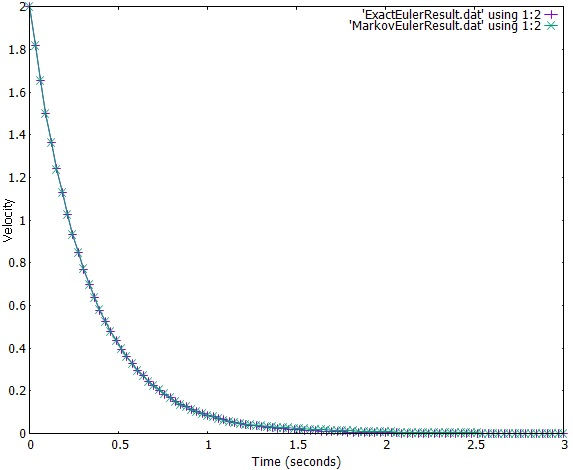
\includegraphics[scale = 0.55]{EulersApproximateStateC++}
	\caption{Euler's approximation method results}
\end{figure}
\begin{figure}[h!]
	\centering
	\label{gnuplot-control}
	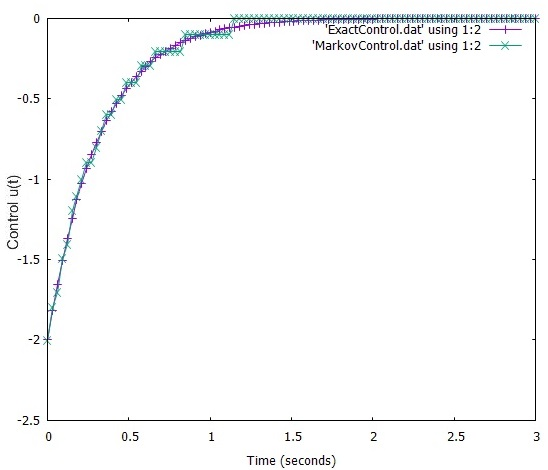
\includegraphics[scale = 0.6]{EulersApproximateControlC++}
	\caption{Euler's approximation method results}
\end{figure}

The benefit of utilising the C++ code base is a dramatic increase in speed: MATLAB would take around 15 seconds to complete the execution and plotting of graphs, where as this new code base takes less than a second to complete.

\newpage

\section{Comparison and Results}
\subsection{Memory usage}
\todo{Why does Continuous decomposition utilise so much memory?}
\subsection{Efficiency and Accuracy}
\todo{how accurate is c3?}
\subsection{Solution Storage Space}

\subsection{Recommendations}

\newpage 

\section{Conclusion}

\newpage

\section{References}
\begin{thebibliography}{9}
	% 1
	\bibitem{dynamicprogramming} 
	R. Bellman
	\textit{Dynamic Programming}. 
	Mineola, New York: Dover Publications Inc., 2003
	
	%2
	\bibitem{powersystem} 
	Power Systems Engineering Research Center
	\textit{Computational Challenges and Analysis under Increasingly Dynamic and Uncertain Electric Power System Conditions}.
	PSERC Publications, 2012
	
	%3
	\bibitem{alex-c3}
	A. Gorodetsky, S. Karaman, Y. Marzouk
	\textit{High-Dimensional Stochastic Optimal Control using Continuous Tensor Decompositions}
	
	%4
	\bibitem{kushner}
	Harold J. Kushner, Paul G. Dupuis
	\textit{Numerical Methods for Stochastic Control Problems in Continuous Time}.
	Springer-Verlag, 1992	
	
	%5
	\bibitem{c3c}
	A. A. Gorodetsky
	\textit{Compressed Continuous Computation Github}.
	[Online] 2016
	https://github.com/goroda/Compressed-Continuous-Computation
	
	%6
	\bibitem{c++film}
	B. Stroustrup
	\textit{The Essence of C++}.
	United Kingdom: University of Edinburgh, 2014
	[Online Film] https://www.youtube.com/watch?v=86xWVb4XIyE\&t=
	
	%7
	\bibitem{c3cs}
	A. A. Gorodetsky
	\textit{Stochastic optimal control using compressed continuous computation Github}.
	[Online] 2016
	https://github.com/goroda/c3sc
	
	%8
	\bibitem{nise}
	N. S. Nise
	\textit{Control Systems Engineering, 7th Ed}.
	Wiley, 2015
	
	%9
	\bibitem{ieeeControl}
	A. E. Bryson 
	\textit{Optimal Control - 1950 to 1985}.
	IEEE Control Systems, vol. 3, no. 16, pp. 26-33, 1996
	
	%10
	\bibitem{costfunction}
	\textit{Cost Function}.
	[Online] Accessed 10 April 2017
	MyAccountingCourse.com
	
	%11
	\bibitem{powell}
	W. B. Powell
	\textit{Approximate Dynamic Programming: Solving the Curses of Dimensionality}.
	United States of America: Wiley, 2017
	
	%12
	\bibitem{wikiDyn}
	\textit{Dynamic Programming}.
	[Online] Accessed 10 April 2017
	https://en.wikipedia.org/wiki/Dynamic\_programming\#cite\_note-1
	
	%13
	\bibitem{chebfun}
	\textit{Chebfun Matlab Package}
	[Online] Accessed September 2017
	http://www.chebfun.org/
	
	%14
	\bibitem{ft-alex}
	A. A. Gorodetsky
	\textit{Function-Train: A continuous analogue of the tensor-train decomposition}.
	[Online] Accessed 2017
	http://www.alexgorodetsky.com/papers/ft\_arxiv.pdf
		
	%15
	\bibitem{thesis} 
	Alex Arkady Gorodetsky
	\textit{Continuous low-rank tensor decompositions, with applications to stochastic optimal control and data assimilation}.
	Department of Aeronautics and Astronautics, at the Massachusetts Institute of Technology
	
	%16
	\bibitem{AlexGorod}
	A. A. Gorodetsky1`
	\textit{Alex Gorodetsky's Website}.
	[Online] 2017
	http://www.alexgorodetsky.com/index.html
	
	%17
	\bibitem{zylong}
	Z. Y. Long, G. Ledwich and J. J. Ford
	\textit{Nonlinear Control of Single-Machine-Infinite-Bus Transient Stability}.
	in Proceedings Power Engineering Society General Meeting, 2006
	
	
\end{thebibliography}
\newpage
\section{Appendix}
\begin{appendices}
	The following two figures depict the original proposal and Gantt chart for the breakdown and timing of this task. In the second semester this had to be adjusted.
	\section{Gantt Chart}\label{app_itemA}
	\[\]
	\[\]
	\[\]
	\begin{figure}[h]
		\centering
		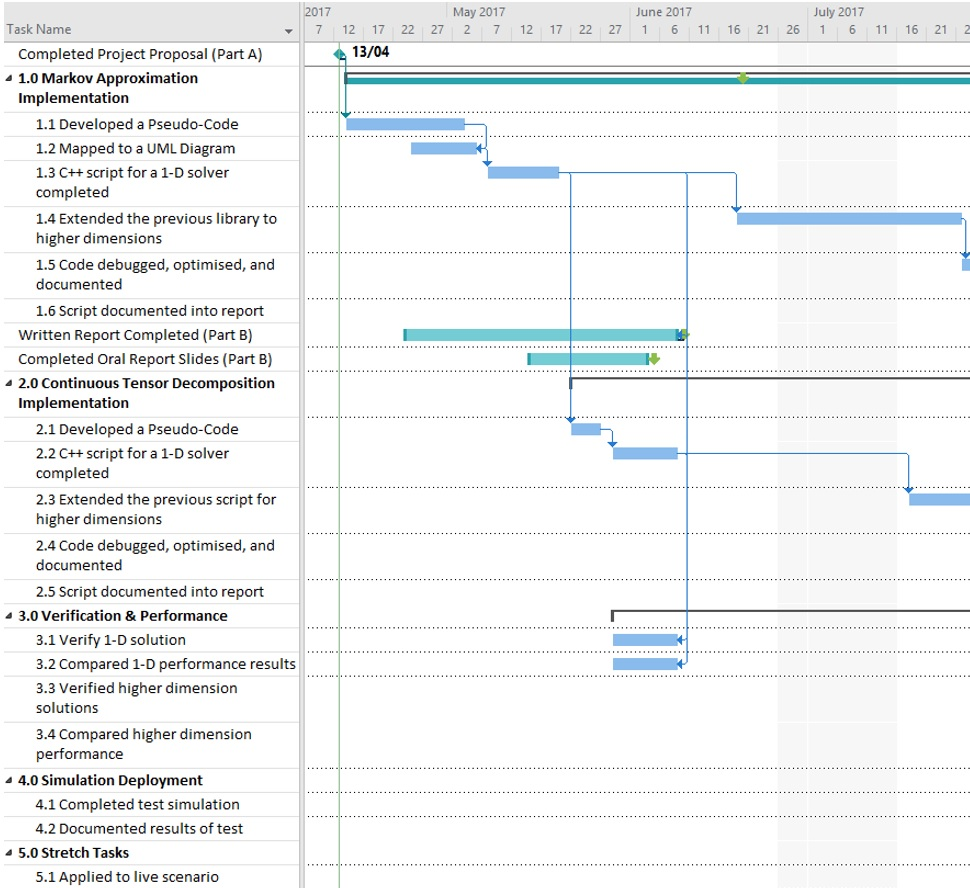
\includegraphics[scale=.6]{OldGanttPart1}
		\caption{Old Gantt Chart Schedule (Part 1)}
	\end{figure}
	\newpage
	\[\]
	\[\]
	\[\]
	\begin{figure}[h]
		\centering
		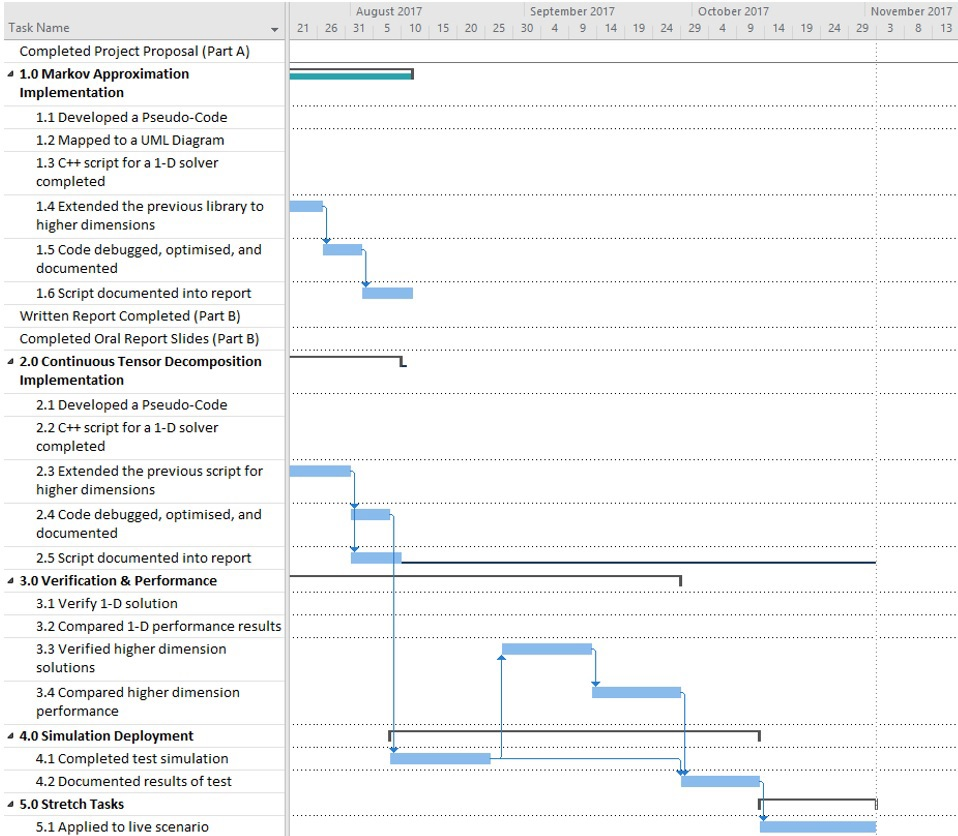
\includegraphics[scale=.6]{OldGanttPart2}
		\caption{Old Gantt Chart Schedule (Part 2)}
	\end{figure}
	\newpage
	As noted, the schedule in the second semester had to be altered to accommodate for extra time in overcoming the obstacles of learning and setting up the C3 library. This new Gantt chart was updated to reflect the status of completion of each task at the time of the second semester (shown by a small blue bar under each task timeline bar) and also has a change in dates. The changes to be noted are: \\
	\begin{itemize}
		\item Times now more closely aligned with actual work hours - meaning a single day now meant a solid days amount of work (whereas before a week was given to say -- within that week this task should be done).
		\item Changed lengths for Tasks 2.1 and 2.2 to 2 days and 4 days respectively. This was done because it became clear that the some Pseudo code was already present in the continuous decomposition library. Also, the C++ script development is quite intuitive once the pseudo code is understood.
		\item Changed lengths for both Tasks 3.1 and 3.2 to 1 day. This was done because the verification of 1-dimension solution can be verified very simply using the already developed Euler method and a visual comparison. The performance also would be a fairly simple task to analyse using standard C++ timing templates.
		\item Changed lengths for both Tasks 3.3 and 3.4 to 2 days. Again, this was done because the verification stage would now only be a simple visual comparison of different dimensions.
		\item Changed lengths for both Tasks 4.1 and 4.2 to 2 days. This was done because the development of a library by myself and a working script would mean that I already have a fair idea of how to apply the code to a control problem. \\
	\end{itemize}
	
	All the noted items were also moved forward to align with the date of the adjustment (i.e. they were moved further forward in the schedule).
	\[\]
	\begin{figure}[h!]
		\centering
		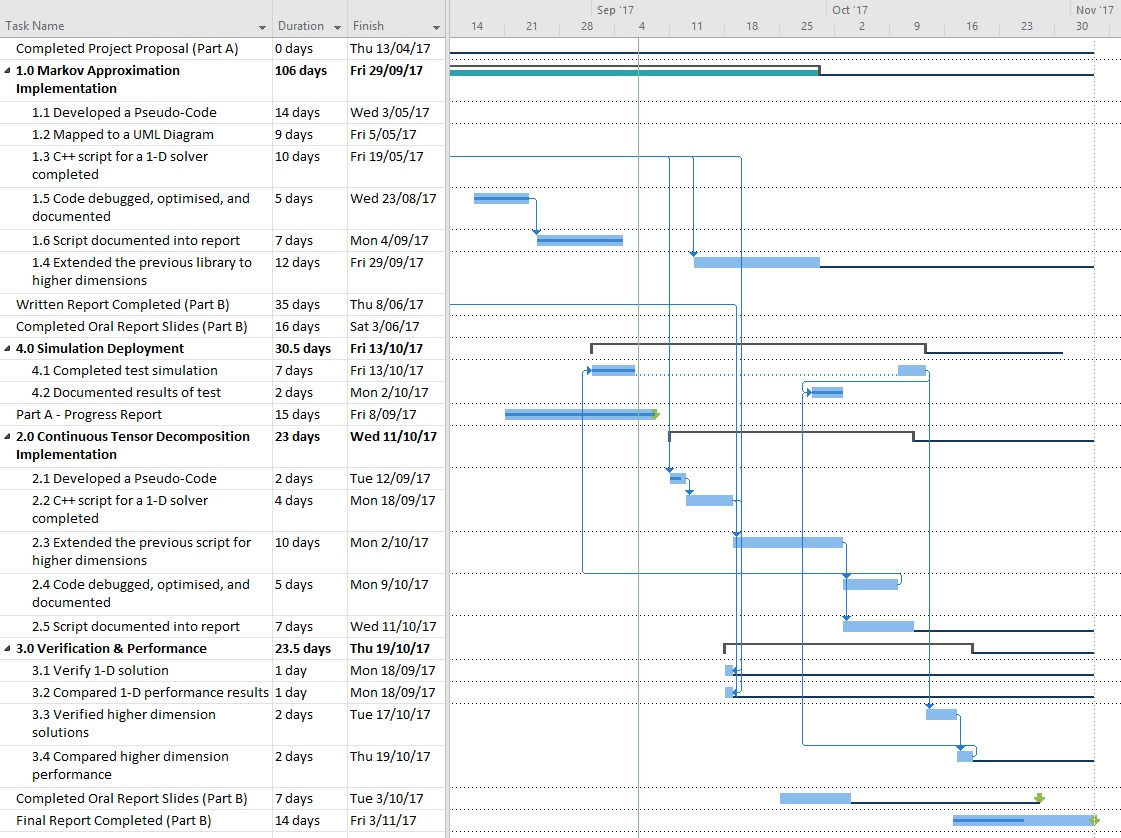
\includegraphics[scale=0.54]{UpdatedGanttProgressSem2}
		\label{UpdatedGanttProgress}
		\caption{Gantt Chart with updated progress}
	\end{figure}

\newpage

	\section{Work Breakdown structure}\label{app_itemB}
	All tasks below were given as part of the original project proposal, and thus the dates and times aligned to the first Gantt Chart given in \todo{Create reference to different gantt charts}
	
	Note that the time frames had originally been put into place to aim for deployment in a real environment at the end of the year, but this ‘real’ deployment is not the key component of this research project. The original schedule also had planned to have a 1-dimensional problem verified and compared using both the MCA method and the continuous decomposition method. This became a harder and longer task than anticipated because of several reasons: \\
	\begin{itemize}
		\item The learning curve for learning the MCA method was tougher than anticipated, and the same applies for learning the continuous decomposition method.
		\item I ran into many problems trying to set up the C3 library on Windows. Thus I had to install another operating system (Ubuntu) and download all the required packages on there before being able to develop. \\
	\end{itemize}
	
	\subsection{Segment 1 - Markov Approximation Implementation}
	\underline{\textbf{Task 1.1 Developed a Pseudo-Code}} \quad 14/4/2017 to 3/5/17 (14 Days) \\
	
	Before developing any code, the fundamentals of the MCA must first be understood. This task has thus been given 14 days to account for the time taken to study and apply this topic. A large part of this study will come from [3]. Also, before developing any C++ code, developing of a pseudo-code will help to establish the required procedures and tasks that will need to be coded -– it will act as a guide to ensure that when code is written, it is only the necessary parts being coded (often programmers can find themselves coding unnecessarily). 
	The learning and developing of Pseudo-Code has not been split into two separate tasks because the best way to understand is to apply what is learnt. Thus, the learning and developing will go hand in hand for 14 days. \\
	Resources: Will need the aforementioned book [3]. Will also need a Git server to store the current code and for future developments to be reviewed by the supervisor. This topic is expected to take quite a while to learn but it has been targeted at 14 days to be able to begin working on the script as soon as possible. \\
		
	\noindent\underline{\textbf{Task 1.2 Mapped to a UML Class Diagram}} \quad 13/4/17 to 5/5/17 (9 Days) \\
	
	A Unified Modelling Language (UML) Class Diagram is the main building block of any object-oriented solution [15]. It displays the classes as a system and therefore can show relationships between classes, their attributes, and their operations. Creating this diagram will further break down the code structure and hopefully express how memory will be managed and how classes will cohesively work together to optimise the code. \\
	Resources: Will need Microsoft Visio. 9 days has been allocated for this task, but this time development time crosses over that of Task 1.1 and thus is expected to be finished shortly thereafter. \\
	
		
	\noindent\underline{\textbf{Task 1.3 C++ script for a 1-D solver completed}} \quad 8/5/17 to 19/5/17 (10 Days) \\
	
	This script is aimed at solving a 1-D stochastic optimal control problem by using the developed library. By creating this script for a lower dimension case, it will help to ensure higher dimension scripts have an example to follow on from. \\
	Resources: An IDE to help develop the code faster, and in conjunction with the library. The current plan is to use Visual Studio Enterprise under a QUT Student License, because of its IntelliSense feature which will help to ensure proper use of the library. A generous 10 days has been assigned to this script to for finding of any faults (and subsequent fixes) in the library code. \\
	
	\noindent\underline{\textbf{Task 1.4 Extended the previous library to higher dimensions}}
	19/6/17 -- 26/7/17 (12 Days)
	As has been clearly stated, this research project is considering high dimension state space problems. Therefore, this 12 days is crucial to ensure that this script functions properly. The higher dimension cases vary from \cite{zylong} to the UAV test bed scenario (but the fundamental concepts for both will be the same).\\
	
	\noindent\underline{\textbf{Task 1.5 Code debugged, optimised, and documented}} \quad 27/7/17 to 2/8/17 (5 Days) \\
	
	This 5-day period is given to revisit libraries and scripts to ensure the code is fully debugged (or for as many bugs as are noticed), optimised (again, for in as many areas as are seen as necessary), and then to ensure the library is documented. There will not be any testing scripts to ensure the full functionality of the library, only the scripts which will be written for it will act as tests. \\
	Resources: Will need to use Doxygen to create a documentation for the library. Documenting can take a long time, so depending on the supervisors need this can take up to 5 days (what has been accounted for) or it can be as simple as 2 days’ worth of work.\\
	
	\noindent\underline{\textbf{Task 1.6 Script documented into report}} \quad 3/8/17 to 11/8/17 (7 Days) \\
	
	The results of running the script will be written into the report as they happen, but this task is to ensure the reader of a report can see a clear correlation between the code and mathematical principles. \\
	Resources: Ideally this should be a continuation of reporting which should occur along the way, but this time of 7 days is to ensure a good quality report (the front-end of the work) is produced.
	
	\subsection{Segment 2 - Continuous Tensor Decomposition Implementation}
	\underline{\textbf{Task 2.1 Developed a Pseudo-Code}} \quad 22/5/17 to 26/5/17 (5 Days) \\
	
	This time is mostly learning and understanding the mathematical concepts.
	Alex has already included a few snippets of Pseudo code in [16], but here we will cover some of the areas he didn’t: we will develop a pseudo code that shows how to utilise his library for an example problem (preparatory for the script). \\
	Resources: Will be looking a lot at [16], [14], and [17]. Might also look to use Code Rocket .NET [18], an extension to Visual Studio IDE which enhances Pseudo-Code development (or something similar). The goal is to work on this immediately after the 1-D script has been written for the MCA Implementation (Task 1.3), thus allowing for a demonstration between the two codes by the first oral presentation. However, the allotted time of 5 days may not be enough.\\
	
	\noindent\underline{\textbf{Task 2.2 C++ script for a 1-D solver completed}} \quad 29/5/17 to 8/6/17 (10 Days) \\
	
	This script will access the C3 and C3SC libraries, and using their Tensor Decomposition method it will be written to solve the same 1-D problem as the MCA 1-D script. Ten days has been allocated to account for the learning of the library. \\
	Resource: Will need to have up-to-date C3 and C3SC libraries from \cite{c3c} and \cite{c3cs} respectively.\\
	
	\noindent\underline{\textbf{Task 2.3 Extended the previous script for higher dimensions}} \quad 18/7/17 to 31/7/17 (10 Days) \\
	
	See Task 1.4 for reason of this task - with the difference being that this is an extension of the Tensor Decomposition script and not the Markov Approximation Script.\\
	
	\noindent\underline{\textbf{Task 2.4 Code debugged, optimised, and documented}} \quad 1/8/17 to 7/8/17 (5 Days) \\
	
	Not the debugging of the library but rather the debugging of the script. Again, the debugging and optimisation will occur on an as-needed basis. The documenting will be a documentation of how the script works (in-code comments) so that a future student could pick up where it has been left off.\\
	
	\noindent\underline{\textbf{Task 2.5 Script documented into report}} \quad 1/8/17 to 9/8/17 (7 Days) \\
	
	Again, it will be important for a reader of the report to be able to see how the mathematical concepts have been mapped to code. Hence, this time is set aside to ensure proper documentation has been completed. \\
	Resources: Will use Microsoft Word or a Latex documentation if there appears to be a lot of mathematical discussion in the content of the report.
	
	
	\subsection{Segment 3 - Verification \& Performance}
	\underline{\textbf{Task 3.1 Verify 1-D solution}} \quad 29/5/17 to 8/6/17 (10 Days) \\
	
	Several methods of verification will happen:
	\begin{enumerate}
		\item Verify that both methods get the same results as that of a simple linear known problem with known solution
		\item Some/brief mathematical verification that the solution to both methods is approximately close
	\end{enumerate}
	Resources: Will need a known problem to test against, perhaps one suggested by supervisor.\\
	
	\noindent\underline{\textbf{Task 3.2 Compared 1-D performance results}} \quad 29/5/17 to 8/6/17 (10 Days) \\
	
	The two main performance criteria to compare will be the time taken to solve the problem, and the storage space required to store the solution. Extra factors will be taken into consideration, such as the time taken to set up/load the problem using either method, and total size of either script and associated libraries. \\
	Resources: Will need to include timing framework into scripts or have a software tool which can time the process independently.\\
	
	\noindent\underline{\textbf{Task 3.3 Verified higher dimension solutions}} \quad 28/8/17 to 12/9/17 (12 Days) \\
	
	Here we verify that the Tensor decomposition technique gets the same result as the MCA for a nonlinear known problem with known solution (the opted problem being \cite{zylong}). After which we also verify that both methods get the same result within the UAV testing bed environment. \\
	Resources: Will need access to the MATLAB to run the UAV testing bed (using the student QUT Student License).\\
	
	\noindent\underline{\textbf{Task 3.4 Compared higher dimension performance}} \quad 13/9/17 to 28/9/17 (12 Days) \\
	
	Again, the two main performance criteria to be compared will be the time taken to solve the problem, and the storage space required to store the solution. Here we also will confirm if either method can store the solution in a file of 8GB or less. The same extra factors will be taken into consideration. Results will be ported to MATLAB to utilise MATLAB’s figure plots. \\
	Resources: Again, will need to include timing framework into scripts or have a software tool which can time the process independently. If time taken to solve problems becomes very large, will need to change scope specification to more powerful computing hardware, and test accordingly.
	
	\subsection{Segment 4 - Simulation Deployment}
	\underline{\textbf{Task 4.1 Completed test simulation}} \quad 8/8/17 to 25/8/17 (14 Days) \\
	
	This test simulation is for both \cite{zylong} and the UAV test bed environment. Because the first test has a known solution, it is utilised to ensure that the scripts and libraries are generating the correct solutions. \\
	The UAV test bed has been developed by Troy Bruggemann at QUT and is a MATLAB Simulink environment for a UAV. Using this test bed, an optimal solution will be generated for a UAV manoeuvring through a tight gap scenario. \\
	Resources: Online access is already provided to the UAV MATLAB Simulink environment, but will have to ensure access is available at the time of testing the simulation.\\
	
	\noindent\underline{\textbf{Task 4.2 Documented results of test}} \quad 29/9/17 to 12/10/17 (10 Days) \\
	
	Here we will be preparing the report which is to be given in Semester 2. The due date for this report has not been given yet but it could be estimated towards the end of the semester (around November). Hence, this documentation has been planned well in advance to allow for further scope evolution and to account for unforeseen delays in the schedule.
	
	\subsection{Milestones}
	\underline{\textbf{Task Completed Oral Report Slides (Part B)}} \quad 15/5/17 to 3/6/17 (16 Days) \\
	
	This oral will take the form of a digital presentation (including slides/poster/videos as appropriate) that will be assessed by the supervisor in a public forum with peers present. In this presentation, the research findings will be briefly explained with an assumption that all present are knowledgeable in the discipline of control systems. \\
	Resources: Will use Microsoft PowerPoint for the presentation, and utilise figures of results plotted from MATLAB. \\
	
	\noindent\underline{\textbf{Task Written Report Completed (Part B)}} \quad 24/4/17 to 8/6/17 (35 Days) \\
	
	This written report will provide a detailed update on the investigation and will present the current analysis, results and findings as of the mid semester point. It will indicate any changes in the project definition and scope and show the changes to the schedule (if any have occurred). The report may also give additional literature review discussion. Ultimately this is a reflection of the progress made so far and what has been learnt. \\
		
	\subsection{Stretch Tasks}
	\underline{\textbf{Task 5.1 Applied to live scenario}} \quad 13/10/17 to 2/11/17 (15 Days) \\
	
	Although the current schedule allows for this live scenario to still occur, it is possible that the current schedule will be rearranged before reaching this point. But if all goes according to plan (or even ahead of schedule) then the goal is to test the results in a live environment - with an actual UAV or a Quadcopter, and have the control devices manoeuvre through a tight gap (at a safe velocity and altitude). \\
	Resources: Access to a test UAV or test Quadcopter, along with camera gear to film (or photograph) the simulation in action, and other necessary recording devices to measure the validity of the solution. 
	\newpage
	
	\section{Brief on Linear Quadratic Regulator (LQR)}\label{app_itemC}
	\subsection{From Modern Control Lecture Notes}
	A functional maps a function into a number
	\begin{align}
	(J:u(t),t\in[0,T]\rightarrow \Real)
	\end{align}
	In the general optimal control problem (OCP), the functional 
	\[ J(x_{0},u(t)) = h(x(T)) + \int_{0}^{T}g(x(t),u(t))dt\]
	measures deviations from the desired performance. Hence, we seek to minimise it.
	
	If the system we are working with is linear, i.e. $ \dot{x} = Ax + Bu$ with $ x(0) = x_{0} $, and the cost functional is quadratic of the form
	\begin{equation}
	J(x_{0}u(t)) = x^{\intercal}(T)Q_{T}x(T) + \int_{0}^{T}(x^{\intercal}Qx(t), u^{\intercal}(t)Ru(t))dt
	\end{equation}
	Then the control will seek to drive the initial state $ x(0) $ to the zero state and keep it there - this is called a regulation problem. The OCP is called infinite horizon LQR problem.
	
	If the system $ \dot{x} = Ax + Bu$ is controllable, then the optimal controller $ u^{*}(t) = -Kx(t) $ minimises the cost functional
	\begin{equation}
	J(x_{0},u) = \int_{0}^{\infty} (x^{\intercal}Qx + u^{\intercal}Ru)dt \qquad Q\ge 0 \quad R > 0
	\end{equation}
	where $ K = R^{-1}B^{\intercal}S $ and $ S $ is the non-negative solution of the Algebraic Riccati Equation:
	\begin{equation}
	S = S^{\intercal}\ge 0: \qquad A^{\intercal}S + SA - (SB)R^{-1}(B^{\intercal}S) + Q = 0
	\end{equation}
	
	\subsection{Ricatti Optimal Control Problem}
	The optimal control can be expressed as
	\begin{equation}
	u^{o}(t) = -\mathbf{K}_{u}(t)x(t)
	\end{equation}
	where $ \mathbf{K}_{u}(t) $ is a time-varying gain given by
	\begin{equation} 
	\mathbf{K}_{u}(t) = \mathbf{\Phi}^{-1}\mathbf{B}^{\intercal}\mathbf{P}(t)
	\end{equation}
	
	We also have 
	\begin{equation}
	\mathcal{W}(x(t), u^{o}(t), t) = x^{\intercal}\left(	\mathbf{\Psi}-\mathbf{P}(t)		\right)
	\end{equation}
	\newpage
	

	
\includepdf[scale = 0.9,pages=1,pagecommand=\section{User Manual for Installing and Running code base}]{../UserManual.pdf}
	
\includepdf[pages=2-]{../UserManual.pdf}
\end{appendices}

\end{document}